\documentclass[11pt]{article}
\usepackage[utf8]{inputenc} % Para caracteres en espa�ol
\usepackage{amsmath,amsthm,amsfonts,amssymb,amscd}
\usepackage{multirow,booktabs}
\usepackage[table]{xcolor}
\usepackage{fullpage}
\usepackage{lastpage}
\usepackage{enumitem}
\usepackage{multicol}
\usepackage{fancyhdr}
\usepackage{mathrsfs}
\usepackage{wrapfig}
\usepackage{setspace}
\usepackage{esvect}
\usepackage{calc}
\usepackage{multicol}
\usepackage{booktabs}% http://ctan.org/pkg/booktabs
\newcommand{\tabitem}{~~\llap{\textbullet}~~}
\usepackage{cancel}
\usepackage{graphicx}
\graphicspath{ {pictures/} }
\usepackage[retainorgcmds]{IEEEtrantools}
\usepackage[margin=3cm]{geometry}
\usepackage{amsmath}
\newlength{\tabcont}
\setlength{\parindent}{0.0in}
\setlength{\parskip}{0.05in}
\usepackage{empheq}
\usepackage{framed}
\usepackage[most]{tcolorbox}
\usepackage{xcolor}
\colorlet{shadecolor}{orange!15}
\parindent 0in
\parskip 12pt
\geometry{margin=1in, headsep=0.5in}
\theoremstyle{definition}
\newtheorem{defn}{Definition}
\newtheorem{reg}{Rule}
\newtheorem{exer}{Exercise}
\usepackage{setspace}
%\singlespacing
%\onehalfspacing
%\doublespacing
\setstretch{1.5}
\newtheorem{note}{Note}
\begin{document}
\setcounter{section}{0}
 \pagestyle{fancy}
\fancyhf{}
\rhead{AE370: Application Problems}
{\LARGE \bf Application Problem 1: Beam Extension}\\ \\
\begin{center}
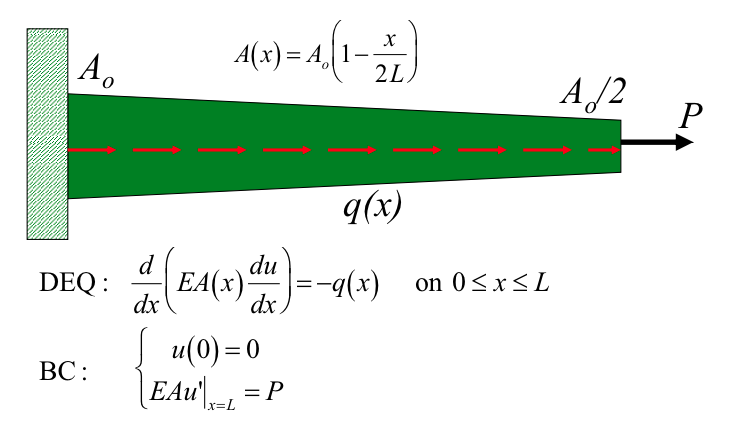
\includegraphics[scale=0.5]{1.png}
\end{center}
\textbf{\begin{itemize}\item Discretize the DEQ with the second-order central finite difference scheme\item Write all the terms entering the resulting linear system, assuming n equally
spaced grid points\item Use two approaches for the BC at x=L\begin{itemize}\item Backward difference scheme\item Ghost cell approach\end{itemize}\end{itemize}} \newline
\noindent\rule{16.5cm}{0.4pt}
\newpage
%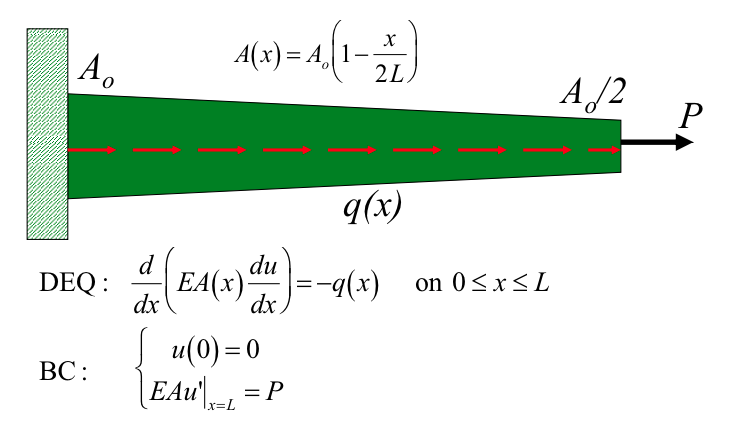
\includegraphics[scale=0.75]{1.png}
\textbf{Discretize the DEQ with the second-order central finite difference scheme}

Further computing the DEQ given provides us with:
\begin{equation*}
\begin{aligned}
\frac{\mathrm{d} }{\mathrm{d} x}\Bigg(EA_o\bigg(1-\frac{x}{2L}\bigg)\frac{\mathrm{d} u}{\mathrm{d} x}\Bigg) = EA_o\bigg(1-\frac{x}{2L}\bigg)\frac{\partial^2 u}{\partial x^2} - EA_o\bigg(\frac{1}{2L}\bigg)\frac{\partial u}{\partial x}
\end{aligned}
\end{equation*}
The \textbf{Second Order Central Difference Scheme} tells us...
\begin{equation*}
\begin{aligned}
\frac{\partial^2 u}{\partial x^2}\bigg|_{i} &= \frac{u_{i+1}-2u_{i}+u_{i-1}}{\Delta x^2} + O(\Delta x^2) \\ \\ 
\frac{\partial u}{\partial x}\bigg|_{i} &= \frac{u_{i+1}-u_{i-1}}{2 \, \Delta x} + O(\Delta x^2)
\end{aligned}
\end{equation*}
Substituting the discretized equations given by the second order central difference scheme, we get
\begin{equation*}
\begin{aligned}
EA_o\bigg(1-\frac{x}{2L}\bigg)\bigg[\frac{u_{i+1}-2u_{i}+u_{i-1}}{\Delta x^2}\bigg] - \frac{EA_o}{2L}\bigg[\frac{u_{i+1}-u_{i-1}}{2 \, \Delta x}\bigg] = -q(x_i)
\end{aligned}
\end{equation*}
Expanding these terms, simplifying the equation and combining like terms, we get an equation in the form
\begin{equation*}
\begin{aligned}
a_i \, u_{i-1} + b_i \, u_{i} +  c_i \, u_{i+1}  = d_i
\end{aligned}
\end{equation*}
Where
\begin{equation*}
\begin{aligned}
a_i &= EA_o\bigg(1-\frac{x_i}{2L}\bigg)\bigg(\frac{1}{\Delta x^2}\bigg) + \frac{EA_o}{4L\Delta x}\\ \\
b_i &= -EA_o \bigg(\frac{2}{\Delta x^2}\bigg) \bigg(1-\frac{x_i}{2L}\bigg)\\ \\
c_i &= \bigg(\frac{EA_o}{\Delta x^2}\bigg)\bigg(1-\frac{x_i}{2L}\bigg) - \bigg(\frac{EA_o}{4L\Delta x}\bigg)\\ \\
d_i &= -q(x_i)\\ \\
\end{aligned}
\end{equation*}
The resulting equation is the final discretized form of the GDE.
\newpage
\textbf{Write all the terms entering the resulting linear system, assuming n equally
spaced grid points}

To begin we know our problem will have the following form...
\begin{equation*}
\begin{bmatrix}
n \times n
\end{bmatrix}
\begin{bmatrix}
u_1 \\
u_2 \\
u_3 \\
\vdots \\
u_{n-1} \\
u_{n} \\
\end{bmatrix}
=
\begin{bmatrix}
n \times 1
\end{bmatrix}
\end{equation*}


We will start with the interior by applying the GDE
\begin{equation*}
\begin{bmatrix}
- & - & - & - & \cdots & -\\
a_{2}  & b_{2}  & c_{2}  & 0 & \cdots & 0 \\
0 & a_{3}  & b_{3} & c_{3}  & \cdots  & 0 \\
\vdots &    & \ddots & \ddots & \ddots & \vdots  \\
0  & \cdots & 0 & a_{n-1}  &  b_{n-1}  & c_{n-1}\\
-  & \cdots  & - & - & - &  -\\

\end{bmatrix}
\begin{bmatrix}
u_1 \\
u_2 \\
u_3 \\
\vdots \\
u_{n-1} \\
u_{n} \\
\end{bmatrix}
=
\begin{bmatrix}
- \\
d_2 \\
d_3 \\
\vdots \\
d_{n-1} \\
- \\
\end{bmatrix}
\end{equation*}

Now lets put in the Boundary Conditions. 

We will start with the displacement boundary conditions $\bf{\color{red}{u(0) = 0}}$
\begin{equation*}
\begin{bmatrix}
\color{red}{1} & \color{red}{0} & \color{red}{0} & \color{red}{0} & \cdots & \color{red}{0}\\
a_{2}  & b_{2}  & c_{2}  & 0 & \cdots & 0 \\
0 & a_{3}  & b_{3} & c_{3}  & \cdots  & 0 \\
\vdots &    & \ddots & \ddots & \ddots & \vdots  \\
0  & \cdots & 0 & a_{n-1}  &  b_{n-1}  & c_{n-1}\\
-  & \cdots  & - & -  & - &-\\

\end{bmatrix}
\begin{bmatrix}
u_1 \\
u_2 \\
u_3 \\
\vdots \\
u_{n-1} \\
u_{n} \\
\end{bmatrix}
=
\begin{bmatrix}
\color{red}{0} \\
d_2 \\
d_3 \\
\vdots \\
d_{n-1} \\
-\\
\end{bmatrix}
\end{equation*}
Implementing our final Boundary Condition is a bit more tricky....
\newpage
\textbf{Implement the boundary condition $\bf{\color{red}{EAu'|_{x=L} = P}}$ using a Backward Difference Scheme}

Lets consider our GDE and BC at $x=L$. At $x=L$, $i = n$ the final row in our matrix. The backward Difference scheme tells us...
\begin{framed}
\textbf{Second Order Backward Difference Scheme}
\begin{equation*}
\begin{aligned}
\frac{\partial f}{\partial x}\bigg|_{i} &= \frac{3\,f_i - 4\,f_{i-1} + f_{i-2}}{2 \, \Delta x} + O(\Delta x^2)
\end{aligned}
\end{equation*}
\end{framed}
which in our case results in
\begin{equation*}
\begin{aligned}
\frac{\partial u}{\partial x}\bigg|_{i=n} &= \frac{3 \, u_{n}-4 \,u_{n-1} + u_{n-2}}{2 \, \Delta x} = \frac{P}{EA}
\end{aligned}
\end{equation*}

The resulting equation is the boundary condition equation ready for implementation.

\begin{equation*}
\begin{bmatrix}
1 & 0 & 0 & 0 & \cdots & 0\\
a_{2}  & b_{2}  & c_{2}  & 0 & \cdots & 0 \\
0 & a_{3}  & b_{3} & c_{3}  & \cdots  & 0 \\
\vdots &    & \ddots & \ddots & \ddots & \vdots  \\
0  & \cdots & 0 & a_{n-1}  &  b_{n-1}  & c_{n-1}\\
0  & \cdots  & 0 & \color{red}{\frac{1}{2 \Delta x}}  & \color{red}{-\frac{2}{\Delta x}}  &  \color{red}{\frac{3}{2\Delta x}}\\

\end{bmatrix}
\begin{bmatrix}
u_1 \\
u_2 \\
u_3 \\
\vdots \\
u_{n-1} \\
u_{n} \\
\end{bmatrix}
=
\begin{bmatrix}
0 \\
d_2 \\
d_3 \\
\vdots \\
d_{n-1} \\
\color{red}{\frac{P}{EA}} \\
\end{bmatrix}
\end{equation*}

\newpage
\textbf{Implement the boundary condition $\bf{\color{red}{EAu'|_{x=L} = P}}$ using the Ghost Cell Approach}

Lets take a moment to consider our GDE and BC at $x=L$. At $x=L$, $i = n$ the final row in our matrix. The  Ghost Cell Approach tells us to...

Consider our Neumann Boundary Condition
\begin{equation*}
\begin{aligned}
\frac{\partial u}{\partial x} \bigg|_{n}=\frac{P}{EA}
\end{aligned}
\end{equation*}
Recall the Second Order Central Difference Scheme:
\begin{equation*}
\begin{aligned}
\frac{\partial f}{\partial x}\bigg|_{i} = \frac{u_{i+1} - u_{i-1}}{2 \, \Delta x} + O(\Delta x)
\end{aligned}
\end{equation*}
Equating these and equating for the ghost cell ($u_{n+1}$) we get:
\begin{equation*}
\begin{aligned}
u_{n+1} = \frac{2 \Delta x \, P}{EA} + u_{n-1}
\end{aligned}
\end{equation*}
Substitute the ghost term into the GDE (thereby eliminating the ghost cell ($u_{n+1}$)).
\begin{equation*}
\begin{aligned}
a_n\, u_{n-1} + b_n \, u_{n} +  c_n \, u_{n+1}  = d_n \quad \rightarrow \quad a_in\, u_{n-1} + b_n \, u_{n} +  c_n \, \Bigg(\frac{2 \Delta x \, P}{EA} + u_{n-1}\Bigg)  = d_n
\end{aligned}
\end{equation*}
Which resolves to be...
\begin{equation*}
\begin{aligned}
u_{n-1} \, (a_n + c_n) + b_n \, u_{n} = d_n -  c_n \, \frac{2 \Delta x \, P}{EA}
\end{aligned}
\end{equation*}

The resulting equation is the boundary condition equation ready for implementation.

\begin{equation*}
\begin{bmatrix}
1 & 0 & 0 & 0 & \cdots & 0\\
a_{2}  & b_{2}  & c_{2}  & 0 & \cdots & 0 \\
0 & a_{3}  & b_{3} & c_{3}  & \cdots  & 0 \\
\vdots &    & \ddots & \ddots & \ddots & \vdots  \\
0  & \cdots & 0 & a_{n-1}  &  b_{n-1}  & c_{n-1}\\
0  & \cdots  & 0 & \color{red}{0}  & \color{red}{a_n + c_n}  &  \color{red}{b_n}\\

\end{bmatrix}
\begin{bmatrix}
u_1 \\
u_2 \\
u_3 \\
\vdots \\
u_{n-1} \\
u_{n} \\
\end{bmatrix}
=
\begin{bmatrix}
0 \\
d_2 \\
d_3 \\
\vdots \\
d_{n-1} \\
\color{red}{d_n - c_n \, \frac{2 \, \Delta x \, P}{EA}} \\
\end{bmatrix}
\end{equation*}

\end{document}